\documentclass[catalan, a4paper, nobib]{tufte-handout}

% encoding
\usepackage[utf8]{inputenc}
\usepackage[T1]{fontenc}
\usepackage{lmodern}
\usepackage{babel}

\frenchspacing
\usepackage[style=spanish]{csquotes}
\MakeAutoQuote{«}{»}

\usepackage{booktabs}
\usepackage{circuitikz}
\usepackage{siunitx}
\usepackage{amsmath}

\graphicspath{
    {fotos/}
}

% hyperlink setup / metadata
\usepackage{hyperref}
\AfterPreamble{\hypersetup{
  %%pdfauthor={},
  %%pdftitle={},
  %%pdfsubject={},
}}

% document metadata
\author{Víctor Méndez}
\title{ICOM: Pràctica 2}
\date{14-3-2024}

\begin{document}

\maketitle

\newthought{Activitat 2.1}

El nivell de soroll mesurat és \qty[qualifier-mode = combine]{-105}{\deci\bel\of{m}} per tant el meu SA té una sensitivitat de \qty[qualifier-mode = combine]{-75}{\deci\bel\of{m}}.

Per fer la mesura seleccionem una freqüència central i una amplada de banda (RBW) típica d'un receptor. Un receptor no ha de fer cap sweep en freqüència per tant es posa zero-span. Una VBW baixa ens permet veure la potencia mitjana del soroll. És important posar l'atenuació a \qty{0}{\deci\bel} per tal de no amplificar el soroll a la sortida del mesclador, que és el soroll que estem mesurant.

\newthought{Activitat 2.2}

Segons les mesures fetes (veure la figura \ref{fig:p2}) es calcula que el TOI val \qty[qualifier-mode = combine]{8.8}{\deci\bel\of{m}}.

\marginnote{
    S'ha fet servir la formula demostrada a l'estudi previ.
    \begin{equation}
        TOI=P_{in} + \frac{\Delta}{2}
    \end{equation}
    On $\Delta$ val la diferencia entre $P_{in}$ i la potència d'intermodulació, \qty[qualifier-mode=combine]{60.5}{\deci\bel\of{m}}.
}

Abans de fer cap càlcul es comprova que el mesclador no estigui en zona de saturació. Per fer-ho augmentem l'atenuació i observem la sortida. Si els pics augmenten significa que el mesclador no estava en zona lineal. Òbviament, si el mesclador no està saturat canviar l'atenuació no ha de tenir cap efecte a la sortida doncs la potència d'entrada és la mateixa.

\begin{figure*}[h]
    \begin{center}
        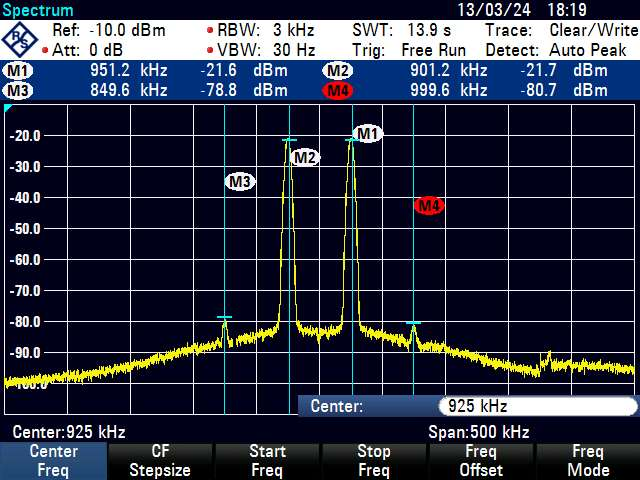
\includegraphics[width=415px]{p2.png}
    \end{center}
    \caption{Visualització de dos tons i els seus productes d'intermodulació}
    \label{fig:p2}
\end{figure*}

\newpage

\newthought{Activitat 2.3}

El soroll fa que sigui impossible efectuar una mesura a \qty{-60}{\deci\bel}, la substituirem per una a \qty{-50}{\deci\bel}.

Una entrada sinusoidal ens permet veure la resposta del filtre per què la seva transformada és una delta, en fer un sweep el resultat és la forma del filtre.

El ràtio entre la amplada a \qty{-50}{\deci\bel} i \qty{-3}{\deci\bel} és $\simeq\num{4}$.

\vspace{30px}

\begin{table*}[h]
    \begin{center}
      \begin{tabular}{@{}rcccccc@{}}
        \toprule
        Desnivell de potència & \qty{-3}{\deci\bel} & \qty{-5}{\deci\bel} & \qty{-10}{\deci\bel} & \qty{-20}{\deci\bel} & \qty{-30}{\deci\bel} & \qty{-50}{\deci\bel} \\
        \midrule
        Amplada de banda & \qty{10}{\kilo\hertz} & \qty{12.857}{\kilo\hertz} & \qty{18.214}{\kilo\hertz} & \qty{25.714}{\kilo\hertz} & \qty{31.548}{\kilo\hertz} & \qty{39.713}{\kilo\hertz} \\
        \bottomrule
      \end{tabular}
    \end{center}
    \vspace{5px}
    \caption{Mesures de l'amplada de banda}
    \label{tab:t1}
\end{table*}

\vspace{30px}

\begin{figure}[h]
    \begin{center}
        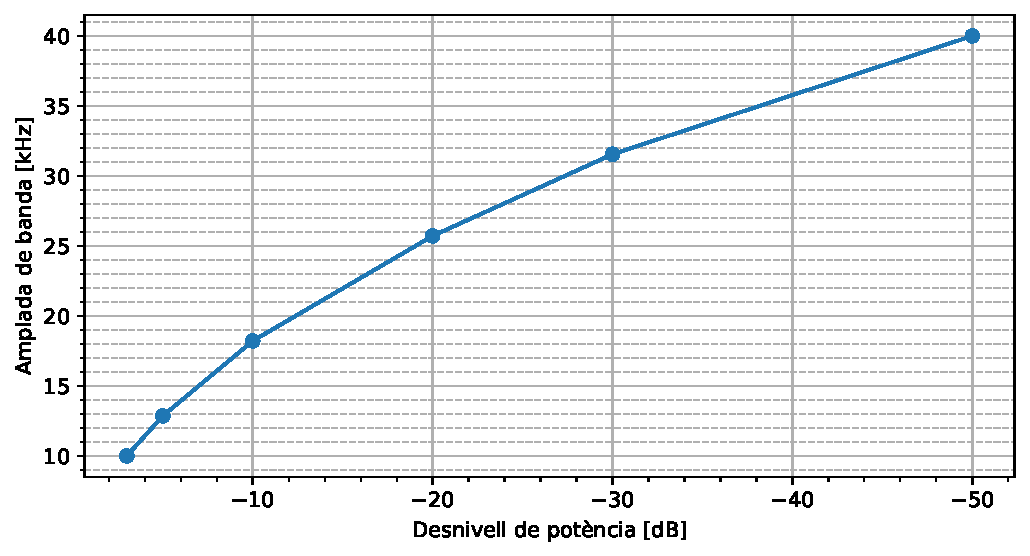
\includegraphics[width=300px]{p3_2.pdf}
    \end{center}
    \caption{Amplada de banda en funció de desnivell de potència}
    %\label
\end{figure}

\begin{figure}[h]
    \begin{center}
        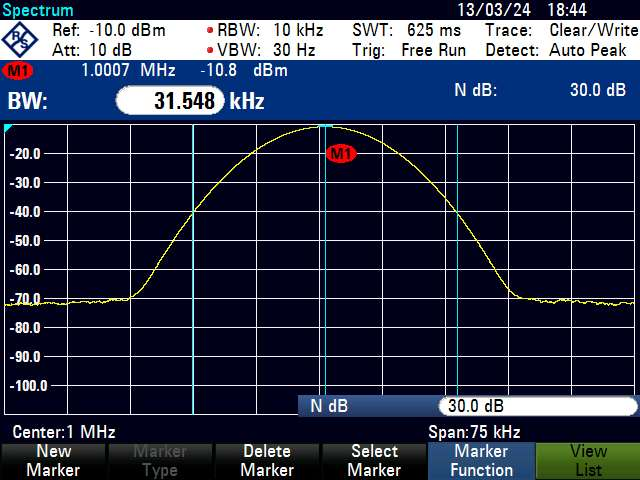
\includegraphics[width=300px]{p3.png}
    \end{center}
    \caption{Visualització de filtre IF}
    %\label
\end{figure}

\end{document}